\chapter{Einleitung} \label{chap:einleitung}

\section{Vorstellung der Flaviviridae-Virusfamilie}
\label{sec:vorstellung-der-flaviviridae-virusfamilie}

Die Flaviviridae stellen eine der größten und vielfältigsten Familien von human- und tierpathogenen RNA-Viren dar \autocite{Simmonds2017}. Zu den wichtigsten klinischen Vertretern gehören Erreger wie das Dengue-Virus, Gelbfieber-Virus, Zika-Virus und das Hepatitis-C-Virus \autocite{Mackenzie2004}. Diese Virenfamilie unterteilt sich in die vier etablierten Gattungen: \textit{Flavivirus}, \textit{Pestivirus}, \textit{Pegivirus} und \textit{Hepacivirus} \autocite{Simmonds2017}. Die jüngere Entdeckung von Jingmenviren und sogenannten Large Genome Flaviviruses (LGFs) hat die evolutionäre Vielfalt der Flaviviridae zusätzlich erweitert und verdeutlicht deren dynamische Anpassungsfähigkeit \autocite{shiDivergentVirusesDiscovered2015}. Die Identifikation von flavivirid Sequenzen in marinen Wirbellosen und basalen Wirbeltierlinien deutet darauf hin, dass die Evolution der Flaviviridae möglicherweise der Evolution der Metazoa durch Virus-Wirt-Kodivergenz über einen Zeitraum von Hunderten von Millionen Jahren folgt.

Glycoproteine spielen innerhalb der Flaviviridae eine Schlüsselrolle, da sie entscheidend den Eintritt des Virus in Zielzellen vermitteln und somit Wirtsspezifität und Pathogenität beeinflussen \autocite{Mukhopadhyay2005}.

\begin{figure}[H]
    \centering
    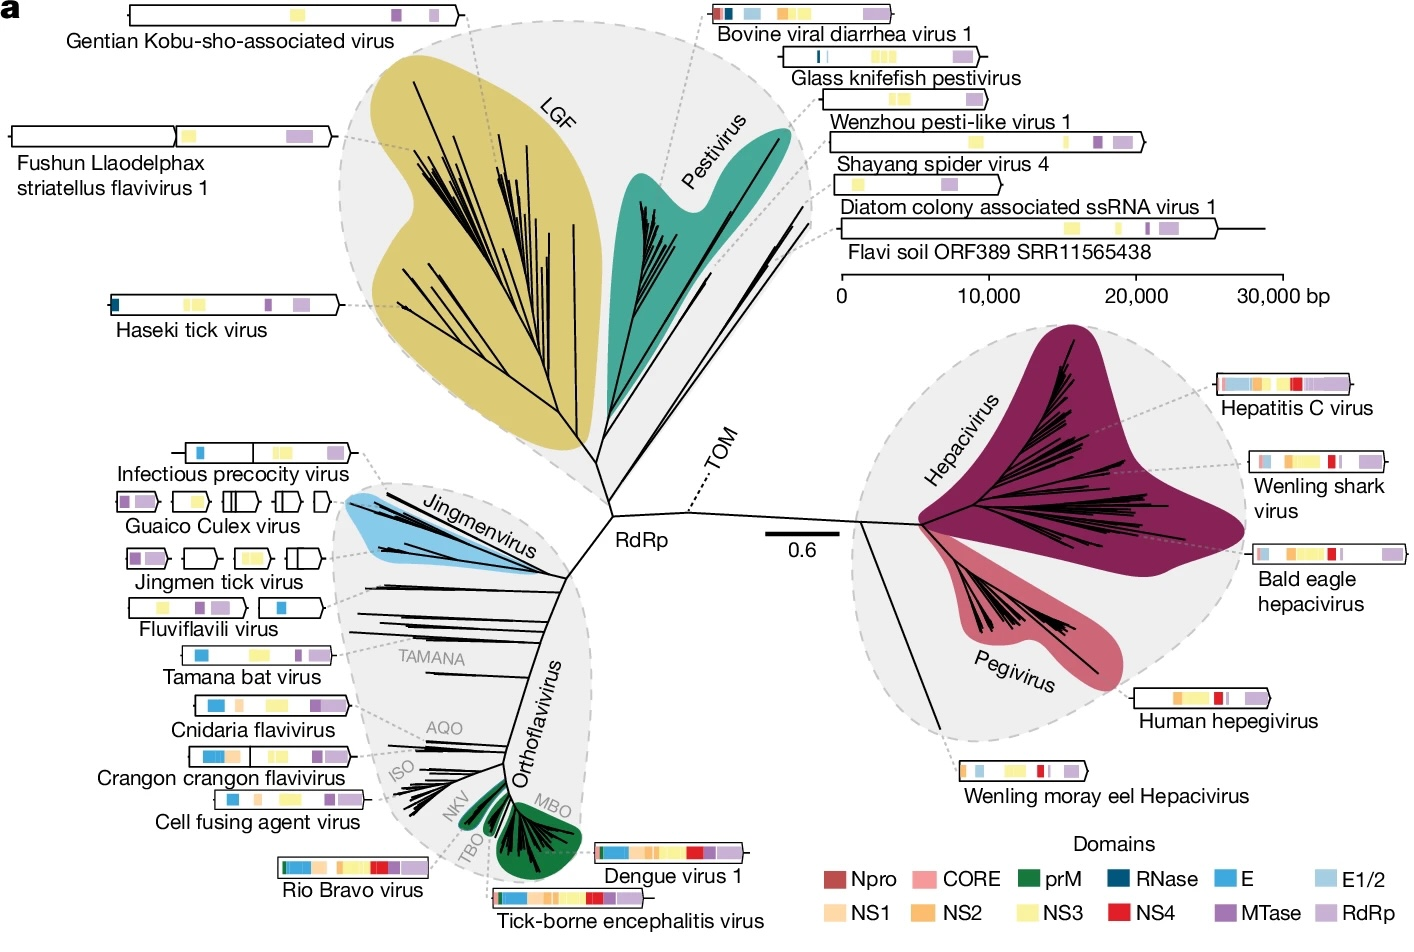
\includegraphics[width=.9\textwidth]{/workspaces/seminar-bioinformatik/images/figure1.jpeg}
    \caption{Protein Foldome der Flaviviridae-Familie.}
    \label{fig:figure1-orginal}
\end{figure}

Die Grafik zeigt die Vielfalt der Flaviviridae-Gattungen, darunter das Orthoflavivirus, Jingmenvirus, LGF und Pestivirus-ähnliche Viren. Die Fusion-Loop-Region ist ein struktureller Bestandteil, der eine zentrale Rolle bei der Membranfusion während des Viruseintritts in die Wirtszelle spielt. Die abgebildeten Schleifen sind farblich kodiert, um die unterschiedlichen Gattungen zu repräsentieren und die strukturellen Gemeinsamkeiten sowie Unterschiede hervorzuheben. Diese Analyse ist essenziell für das Verständnis der evolutionären Beziehungen und funktionellen Diversifikation innerhalb der Flaviviridae-Familie. \autocite{mifsudMappingGlycoproteinStructure2024}

\section{Bedeutung der Glycoprotein-Struktur für Evolution und Pathogenese}
\label{sec:bedeutung-der-glycoprotein-struktur-fuer-evolution-und-pathogenese}

Die Glycoproteine der Flaviviridae erfüllen zentrale Funktionen in der Virusbiologie, insbesondere durch ihre Rolle bei der Membranfusion und der Interaktion mit dem Wirtsimmunsystem \autocite{Heinz2012}. Während das E-Glycoprotein der \textit{Flavivirus}-Gattungen als prototypisches Klasse-II-Fusionsprotein gut charakterisiert ist \autocite{kuhnStructureDengueVirus2002}, weisen die Glycoproteine der Hepaciviren und Pegiviren, insbesondere die E1/E2-Komplexe, einzigartige strukturelle Eigenschaften auf. Diese könnten auf alternative Mechanismen der Membranfusion hindeuten und eine besondere evolutionäre Anpassung darstellen \autocite{Lavie2017}.

Mutationen, Rekombinationen und horizontaler Gentransfer haben entscheidend zur Diversifikation der Glycoprotein-Strukturen beigetragen und somit die Anpassungsfähigkeit der Flaviviridae an unterschiedliche ökologische Nischen gefördert \autocite{Weaver2009}. Die Untersuchung dieser strukturellen Merkmale bietet daher wertvolle Einblicke in die evolutionären Mechanismen, die zur Spezialisierung und Pathogenität der Viren führen. Besonders konservierte Regionen wie die hydrophobe Fusion-Loop-Region und transmembrane Domänen spielen eine zentrale Rolle in der Funktion der Glycoproteine und unterliegen vermutlich starkem Selektionsdruck \autocite{Modis2004}.

\section{Zielsetzung und Vorgehensweise}
\label{sec:zielsetzung-und-vorgehensweise}

Das Ziel dieser Arbeit besteht darin, die evolutionäre Geschichte und die strukturellen Eigenschaften der Glycoproteine der Flaviviridae systematisch zu untersuchen. Aufbauend auf der Arbeit von \textit{Mifsud et al.} \autocite{mifsudMappingGlycoproteinStructure2024} werden bioinformatische Methoden eingesetzt, um die Phylogenie, Proteinstrukturvorhersage und strukturelle Homologien dieser Schlüsselproteine zu analysieren. Hierbei stehen drei zentrale Fragestellungen im Fokus:

Erstens sollen die strukturellen Gemeinsamkeiten und Unterschiede der Glycoproteine zwischen den Gattungen herausgearbeitet werden. Zweitens wird untersucht, welche evolutionären Mechanismen zur Diversifikation dieser Glycoproteine beigetragen haben. Drittens sollen die funktionellen Hinweise, die sich aus konservierten und variablen Strukturmotiven ableiten lassen, analysiert werden.

Die Arbeit gliedert sich wie folgt: Kapitel~\ref{chap:methoden} beschreibt die eingesetzten bioinformatischen Verfahren zur Erstellung von Phylogenien, zur Proteinstrukturvorhersage und zur Homologiesuche. In Kapitel~\ref{chap:ergebnisse} werden die Ergebnisse zu den phylogenetischen Beziehungen und Proteinstrukturen vorgestellt. Kapitel~\ref{chap:diskussion} interpretiert diese Ergebnisse hinsichtlich ihrer evolutionären und funktionellen Bedeutung sowie methodischer Limitationen. Abschließend fasst Kapitel~\ref{chap:schlussfolgerung} die zentralen Erkenntnisse zusammen und gibt einen Ausblick auf zukünftige Forschungsansätze.